\chapter{The Software Build Process}
%Die Aufgabe des Erstellungs- (od. Build)-Prozesses in der
%SW-Entwicklung ist es, die
%benötigten Produkte (Artefakte) in einer konsistenten,
%reproduzierbaren und soweit wie möglich
%automatisierten Weise zu erstellen.

Build is the process of creating the application program for a
software release, by taking all the relevant source code files
and compiling them and then creating a build artefact, such as
binaries or executable program, etc.\\

The build process should be automated as much as possible and
be reproducible.\\

You can also say that the build process is a combination of
several activities which varies for each programming language
and for each operating system but please remember the basic
concepts are universal.\\

\vspace{3mm}

The build process could include the following activities:

%In der Regel umfasst
%dieser Prozess die folgenden Schritte:

\begin{itemize}
\item Fetching the code from source control repository
\item Compile the code and check dependencies
\item Run automated unit tests
\item Link the libraries, code etc accordingly
\item Build artifacts
\item Deploy application
\item Generate documentation
\item Archive build logs
\end{itemize}

To have the possibility to create an automated and reproducible
process, a description of each software (e.g. compiler) including
parameters and dependencies is needed.\\

\vspace{3mm}

The build process is \structure{CRISP} oriented.

%Der Erstellungsprozess soll sich am Prinzip \structure{CRISP} orientieren:

 {\bfseries C}omplete {\bfseries R}epeatable {\bfseries I}nformative {\bfseries S}chedulable {\bfseries P}ortable

Typical tools which could be used are::
\begin{itemize}
\item make, CMake and Automake/Autotools (Unix, Windows/Cygwin)
\item Apache Ant
\item Apache Maven
\item Gradle
\end{itemize}
%
\section{Apache Ant}
Apache Ant is a Java library and command-line tool whose mission
is to drive processes described in build files as targets and
extension points dependent upon each other. The main known usage
of Ant is the build of Java applications. Ant supplies a number of
built-in tasks allowing to compile, assemble, test and run Java
applications. Ant can also be used effectively to build non Java
applications, for instance C or C++ applications. More generally,
Ant can be used to pilot any type of process which can be described
in terms of targets and tasks.\\

\vspace{3mm}

To use Apache Ant, a build file in XML format is needed. This file
has the following prooperties:

%Um Ant zu verwenden, muss eine sogenannte Build-Datei in XML-Format erstellt
%werden. Diese Datei hat folgende Eigenschaften:
\begin{itemize}
\item Each build file contains one project
\item Each project contains one or more {\bfseries Targets}. Each Target
will execute a given number of {\bfseries Tasks}.
\end{itemize}
\newslide
Sample build file:
\begin{lstlisting}[language=xml,morekeywords={project,target,javac,mkdir}]
<project name="SimpleProject" default="compile">

  <target name="init">
    <mkdir dir="build"/>
  </target>

  <target name="compile" depends="init">
    <javac srcdir="src"
        destdir="build"/>
  </target>
</project>
\end{lstlisting}
\ifslides
\else
This build files takes care that
%Die obige Datei sorgt dafür, dass
\begin{enumerate}
\item the directory \verb|build| will be created (if not already there).
\item all Java source code files which are in the \verb|src| directory
  will be compiled and the result will be written to the \verb|build| directory.
\end{enumerate}
\fi
\newslide
%Ein Ant-Prozess kann wie folgt angestossen werden:
A process based on Ant could be started in the following way:

\begin{tabularx}{\linewidth}{l|X}
Call   & Description \\
\hline
ant  &  will execute the default target in the build file (build.xml)\\
%\hline
ant -f otherbuild.xml & using a different name for the build file: otherbuild.xml\\
%\hline
ant compile & executes the target {\bfseries compile}
  aus.\\
%\hline
ant -projecthelp & displays all available targets\\
%\hline
ant -version & displays the current Ant version\\
%\hline
ant -emacs & creates Emacs based log statements.\\
\end{tabularx}

Per default, Ant contains about 80 tasks. Most of the work which
needs to be done in the build process could be covered with the
default tasks. Default tasks are:
\begin{itemize}
\item Copy
\item Create directory
\item Create jar file
\item Compile code
\item Execute operating system command
\end{itemize}
There is also the possibility to extend Ant with your own tasks.
Many extension projects are available.

%Standardmässig bringt Ant über 80 Tasks mit, die einen breiten
%Anwendungsbereich abdecken und die auch durch eigene Tasks erweitert werden
%können. Es gibt über 100 Erweiterungsprojekte und Tools zu Ant.
%
\newslide
\subsection{Constants}
Whenever possible, make use of properties in your build file:
%Um allenfalls notwendige Anpassungen zu vereinfachen, sollten in der
%Build-Datei Konstanten als sogenannte Properties vereinbart werden:
\begin{lstlisting}[language=xml, morekeywords={property,target,javac}]
<property name="build.dir" value="build"/>
<target name="compile">
  <javac srcdir="src"
        destdir="${build.dir}"/>
</target>
\end{lstlisting}
%$
Properties could be defined in an additional file or in the build file
directly:
%Oft sind diese auch in einer separaten Datei definiert:
\begin{lstlisting}[language=xml,morekeywords={property}]
<property file="project.properties"/>
\end{lstlisting}
The project.properties file contains key value pairs:
%In der Datei project.properties sind die Werte zeilenweise aufgeführt:
\begin{verbatim}
build.dir=build
\end{verbatim}
%
\newslide
\subsection{Create Jar file}
A jar file could be created with the jar task:
%Eine Archiv-Datei kann mit dem Task jar erstellt werden:
\begin{lstlisting}[language=xml,morekeywords={target,jar,mkdir}]
<target name="dist" depends="compile"
   description="generate the distribution" >
   <mkdir dir="dist" />
   <jar destfile="dist/project.jar"
        basedir="${build.dir}"/>
</target>
\end{lstlisting}
%$
The attribute destfile defines the final file name and the
basedir defines, which files should be included.


%Das Attribut destfile legt den Filenamen fest und mit basedir wird
%das Verzeichnis bezeichnet, dessen Dateien in die Archiv-Datei
%aufgenommen werden.

\newslide
To create an executable jar file, the following manifest needs to be
added:
%Um eine Archiv-Datei ausführbar zu machen, muss eine Manifest-Datei
%mit folgendem Inhalt hinzugefügt werden:
\begin{verbatim}
  Main-Class: classname
\end{verbatim}
classname is the class, which contains the \verb|main| method. There
is a possibility to do that directly in the Ant task:
%wobei \verb+classname+ die Klasse bezeichnet, welche die Main-Methode
%enthält. In der Ant-Build-Datei kann dies mit dem Element manifest
%vereinbart werden:
\begin{lstlisting}[language=xml,morekeywords={jar,manifest,attribute}]
   <jar destfile="dist/project.jar"
        basedir="${build.dir}">
      <manifest>
	<attribute name="Main-Class"
		   value="example.Main"/>
      </manifest>
   </jar>
\end{lstlisting}
%$
\newslide
\subsection{Fileset}
Filesets are used as a common way to bundle files:
%Mit Filesets können Dateien gruppiert werden:
\begin{lstlisting}[language=xml,morekeywords={fileset,include,exclude}]
<fileset dir="src">
  <include name="**/*.java"/>
  <exclude name="**/*Test*"/>
</fileset>
\end{lstlisting}
A group will be created, containing all files from the \verb|src| directory ending with \verb|.java|
or containing the word \verb|Test| in the filename.
%Hiermit wird eine Gruppe gebildet mit allen Java-Dateien, die im
%src-Verzeichnis und darunter liegen und nicht den Text ''Test'' im
%Namen enthalten.
%
\newslide
\subsection{Path}
A path is a collection of resources (files). A path has an id and could
then be used within another task:
%Als Pfad bezeichnet man eine Sammlung von Ressourcen (Dateien), die
%üblicherweise mit einem Id-Attribut eindeutig gekennzeichnet werden:
\begin{lstlisting}[language=xml,morekeywords={path,pathelement,fileset,include}]
<path id="compile.classpath">
  <fileset dir="lib">
    <include name="**/*.jar"/>
  </fileset>
</path>

<path id="run.classpath">
  <pathelement location="${build.dir}"/>
  <path refid="compile.classpath"/>
</path>
\end{lstlisting}
%$
\newslide
This approach is used to set the classpath in the compilation process:
%Damit kann beim Compilieren der Klassenpfad wie folgt gesetzt werden:
\begin{lstlisting}[language=xml,morekeywords={javac,classpath}]
<javac ...>
  <classpath refid="compile.classpath"/>
</javac>
\end{lstlisting}
%
\newslide
\subsection{Exercise}
\begin{enumerate}
\item Create an Ant build file for the loader project. This build file
should contain the following targets:
\begin{itemize}
\item clean (delete all generated artifacts)
\item compile (compiles the java code)
\item dist (creates an executable jar file, containing the build date)
\end{itemize}

\end{enumerate}
%
\newslide
\subsection{Software and further Informations}
\begin{itemize}
\item Java Development with Ant (Erik Hatcher, Steve Loughan), Manning
  Publications
\item The Apache ANT Project:
  \href{http://ant.apache.org}{ant.apache.org}
\item Apache Ant:
  \href{http://en.wikibooks.org/wiki/Programming:Apache_Ant}
     {en.wikibooks.org/wiki/Programming:Apache\_Ant}
\item Ant Wiki:
  \href{http://wiki.apache.org/ant/FrontPage}{wiki.apache.org/ant/FrontPage}
\item Introduction to
  Ant:\href{http://www.exubero.com/ant/antintro-s5.html}
{www.exubero.com/ant/antintro-s5.html}
\end{itemize}
%
\newslide
%
% http://pettermahlen.com/2010/05/01/code-sharing-use-maven/
%

\newpage

\section{Maven}

Apache Maven is a software project management and comprehension tool.
Based on the concept of a project object model (POM), Maven can manage a
project's build, reporting and documentation from a central piece of
information.\\
Maven’s primary goal is to allow a developer to comprehend the
complete state of a development effort in the shortest period of
time. In order to attain this goal, Maven deals with several areas
of concern:
\begin{itemize}
\item Making the build process easy\\
While using Maven doesn’t eliminate the need to know about the underlying mechanisms, Maven does shield developers from many details.
\item Providing a uniform build system\\
Maven builds a project using its project object model (POM) and a set of plugins. Once you familiarize yourself with one Maven project, you know how all Maven projects build. This saves time when navigating many projects.
\item Providing quality project information\\
Maven provides useful project information that is in part taken from your POM and in part generated from your project’s sources. For example, Maven can provide:
\begin{itemize}
\item Change log created directly from source control
\item Cross referenced sources
\item Mailing lists managed by the project
\item Dependencies used by the project
\item Unit test reports including coverage
\end{itemize}
Third party code analysis products also provide Maven plugins that add their reports to the standard information given by Maven.
\item Encouraging better development practices\\
Maven aims to gather current principles for best practices development and make it easy to guide a project in that direction.\\
For example, specification, execution, and reporting of unit tests are part of the normal build cycle using Maven. Current unit testing best practices were used as guidelines:
\begin{itemize}
\item Keeping test source code in a separate, but parallel source tree
\item Using test case naming conventions to locate and execute tests
\item Having test cases setup their environment instead of customizing the build for test preparation
\end{itemize}
Maven also assists in project workflow such as release and issue management.\\
Maven also suggests some guidelines on how to layout your project’s directory structure. Once you learn the layout, you can easily navigate other projects that use Maven.\\
While takes an opinionated approach to project layout, some projects may not fit with this structure for historical reasons. While Maven is designed to be flexible to the needs of different projects, it cannot cater to every situation without compromising its objectives.
\end{itemize}

%
\subsection{Project Object Model POM}
The pom.xml file is the core of a project's configuration in Maven.
It is a single configuration file that contains the majority of
information required to build a project in just the way you want.\\
The most important information is:
\begin{itemize}
\item \structure{General information}: Project information, Package \ldots
\item \structure{Dependencies}: Dependencies to external libraries,
\item \structure{Build}: information for the build process (plugins),
\item \structure{Properties}: project specific properties (e.g. Java version),
\item \structure{Profile}: Build variants (e.g. PROD, DEV, TST),
\item \structure{Repositories}: 3rd party repositories
\item Reporting: Documentation
\end{itemize}
All information is stored in a file called \verb|pom.xml|:
\begin{lstlisting}[language=xml,
   morekeywords={modelVersion,groupId,artifactId,
   packaging,version,name,url,dependencies,dependency,scope,project}]
  <project xmlns="http://maven.apache.org/POM/4.0.0"
       xmlns:xsi="http://www.w3.org/2001/XMLSchema-instance"
       xsi:schemaLocation="http://maven.apache.org/POM/4.0.0
                  http://maven.apache.org/maven-v4_0_0.xsd">
  <modelVersion>4.0.0</modelVersion>

  <groupId>example</groupId>
  <artifactId>myapp</artifactId>
  <packaging>jar</packaging>
  <version>1.0-SNAPSHOT</version>

  <name>My First App</name>
  <url>http://maven.apache.org</url>

  <dependencies>
  <dependency>
    <groupId>org.junit.jupiter</groupId>
    <artifactId>junit-jupiter-engine</artifactId>
    <version>5.7.1</version>
    <scope>test</scope>
  </dependency>
  <dependency>
    <groupId>org.junit.jupiter</groupId>
    <artifactId>junit-jupiter-api</artifactId>
    <version>5.7.1</version>
    <scope>test</scope>
  </dependency>
  </dependencies>
</project>
\end{lstlisting}
\newslide
General information will be described in the following way:
%Die allgemeinen Angaben werden mit den folgenden Elementen beschrieben:
\begin{itemize}
\item \structure{groupId}: unique identifier of the project organization, e.g. ch.fhnw.mscmi
\item \structure{artifactId}: unique identifier of the outcome (product)
\item \structure{version}: version of the artifact
\item \structure{packaging}: package type (e.g. war, jar)
\item \structure{name}: project name for the documentation
\item \structure{url}: website of the project
\end{itemize}
As a dependency there is the \verb|Junit| framework listed. Other
dependencies could be added (e.g. Apache Commons).\\
A dependency could have a scope (test, compile, provided, runtime, system) to
define the usage area.
%Unter dependencies findet man
%das junit-Artefakt, welches im Projekt für die Test-Phase
%benötigt wird. Hier können weitere Dependency-Elemente
%hinzugefügt mit Scope den jeweiligen Verwendungsbereich
% (test, compile, provided, runtime, system) vereinbart werden.
%
% Lat. ars „Bearbeitung“ und factum „das Gemachte“
% Artefakt:
% in der Softwareentwicklung ein Produkt, das als Zwischen- oder
% Endergebnis der Softwareentwicklung entsteht
%
\newslide
% http://www.avajava.com/tutorials/lessons/what-are-the-phases-of-the-maven-default-lifecycle.html
\subsection{Build-Lifecycle}
The build process in Maven contains the following phases:
%Leicht vereinfacht ist der Build-Prozess bei Maven
%in die folgenden Phasen gegliedert:
\begin{itemize}
\item \structure{compile}: compile the source code
\item \structure{test}: run unit tests
\item \structure{package}: package compiled source code into the distributable format (jar, war, …)
\item \structure{integration-test}: process and deploy the package if needed to run integration tests
\item \structure{install}: install the package to a local repository
\item \structure{deploy}: copy the package to the remote repository
\end{itemize}
%Diese Phasen werden in der dargestellten Reihenfolge durchgeführt. Das
%heisst, wenn man zum Beispiel \verb+package+ ausführen lassen möchte,
%werden zuerst die davor liegenden Phasen validate, compile, und test
%ausgeführt.
%
There are additional goals available:
\begin{itemize}
\item \structure{clean}: deletes all generated files
\item \structure{site}: creates the project documentation
\end{itemize}
\newslide
For the full list of each lifecycle's phases, check out the Maven Reference.

\vspace{3mm}

To create a jar file, the following 8 phases are included:

\begin{tabularx}{\linewidth}{llll}
  & Phase &  Plugin & Goal\\
\hline
1 & process-resources & maven-resources-plugin & resources:resources\\
2 & compile & maven-compiler-plugin & compiler:compile\\
3 & process-test-resources & maven-resource-plugin & resources:testResources\\
4 & test-compile & maven-compiler-plugin & compiler:testCompile\\
5 & test & maven-surefire-plugin  & surefire:test\\
6 & package & maven-jar-plugin & jar:jar\\
7 & install & maven-install-plugin & install:install\\
8 & deploy & maven-deploy-plugin & deploy:deploy\\
\end{tabularx}
%
\newslide
\subsection{How to use Maven?}
A simple example will explain how Maven could be used:
\begin{enumerate}
\item \underline{Create project (based on a template):}
\begin{lstlisting}
mvn archetype:generate
  -DarchetypeArtifactId=maven-archetype-quickstart
  -DarchetypeVersion=1.4
\end{lstlisting}
Some information is needed to create the project. This information
could be provided as parameters or in an interactive mode:

  \begin{itemize}
  \item \structure{groupId}: namespace, organization name
  \item \structure{artifactId}: project identifier
  \item \structure{version}: version identifier
  \item \structure{package}: default package
  \begin{figure}[H]
  \begin{center}
  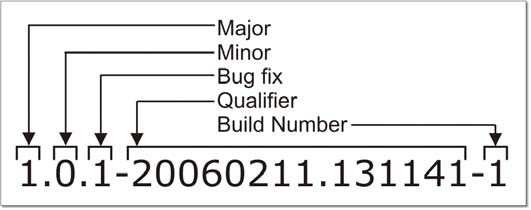
\includegraphics[width=0.65\linewidth]{config-management/major-minor}
  \end{center}
  \caption{Format of the version identifier (Source: Better Builds with Maven)}
  \end{figure}
\newslide
Examples for version identifier:
  \begin{itemize}
  \item 1.0.1-20080211.131141-1
  \item 1.0-alpha
  \item 1.0
  \end{itemize}
  \end{itemize}

A project is now generated with the following file/directory structure:
%Hiermit ist nun die in Abbildung \ref{fig:maven-dirstruct} gezeigte
%Verzeichnisstruktur entstanden.
\begin{figure}[H]
  \centering
\ifslides
  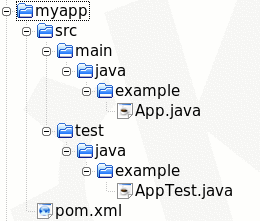
\includegraphics[width=0.4\linewidth]{config-management/maven-dirstruct}
\else
  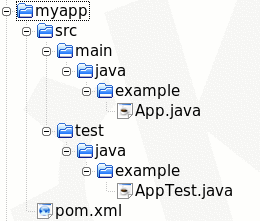
\includegraphics[width=0.4\linewidth]{config-management/maven-dirstruct}
\fi
  \caption{Directory structure of a Maven project}
  \label{fig:maven-dirstruct}
\end{figure}
\newslide
The available project templates could be displayed with the command
\verb|archetype:generate|. The option \verb|-Dfilter| could be used search
for specific templates.
%Mit archetype:generate wird eine Auswahl möglicher Projektvorlagen präsentiert, die mit dem Argument -Dfilter
%eingegrenzt werden kann.
%
\newslide
\item \underline{Compile and Test}
A specific project phase could now be executed on command line:
\begin{lstlisting}
  mvn test
\end{lstlisting}
All phases from start to \verb|test| will now be executed. That means:
\begin{itemize}
\item Dependencies will be solved
\item Compile source code
\item Execute unit tests
\end{itemize}

The Java version which is defined in the \verb|JAVA_HOME| environment
variable will be used to execute the maven build process.

\vspace{3mm}

Specific compiler flags will be defined in the \verb+maven-compiler-plugin+ plugin:
\begin{lstlisting}[language=xml,
  morekeywords={plugins,plugin,configuration,artifactId,source,target}]
  <plugins>
    <plugin>
      <artifactId>maven-compiler-plugin</artifactId>
      <configuration>
        <source>1.8</source>
        <target>1.8</target>
      </configuration>
    </plugin>
  </plugins>
\end{lstlisting}

\item \underline{Using 3rd/external party libraries}
Additional libraries will be added to the \verb|dependencies| section:
\begin{lstlisting}[language=xml,
    morekeywords={dependency,groupId,artifactId,version,scope}]
<dependency>
   <groupId>org.biojava</groupId>
   <artifactId>core</artifactId>
   <version>1.9.5</version>
</dependency>
\end{lstlisting}
Searching in the Maven repository is possible on the page:
\href{https://search.maven.org}{search.maven.org}

Maven will then download the libraries (if not already available) and
stores the files into a local repository.
%
\newslide
\item \underline{Running the program}

Executing a Java application does not belong to the core competencies
of Maven. Nevertheless, there is a possibility to do that:

\begin{lstlisting}
mvn exec:java -Dexec.mainClass=ch.fhnw.mscmi.App
\end{lstlisting}
Additional arguments could be passed with \verb+-Dexec.args=".."+.

The exec plugin could also be configured
\begin{lstlisting}[language=xml,
  morekeywords={plugin,groupId,artifactId,configuration,mainClass}]
<plugin>
  <groupId>org.codehaus.mojo</groupId>
  <artifactId>exec-maven-plugin</artifactId>
  <configuration>
    <mainClass>ch.fhnw.mscmi.App</mainClass>
  </configuration>
</plugin>
\end{lstlisting}
\newslide

\item \underline{Package}
The package command takes the compiled code and package it in its
distributable format, such as a JAR, WAR, EAR.\\
Per default, the dependencies are not included. The assembly plugin could be
used to achieve that:

\begin{lstlisting}[language=xml,
  morekeywords={build,plugins,plugin,artifactId,configuration,descriptorRefs,
  descriptorRef}]
<build>
  <plugins>
    <plugin>
      <artifactId>maven-assembly-plugin</artifactId>
      <configuration>
        <archive>
          <manifest>
            <mainClass>ch.fhnw.mscmi.App</mainClass>
          </manifest>
        </archive>
        <descriptorRefs>
          <descriptorRef>jar-with-dependencies</descriptorRef>
        </descriptorRefs>
      </configuration>
    </plugin>
  </plugins>
</build>
\end{lstlisting}

With the goal {\bfseries assembly:single} the application,
including the dependencies, could be generated.\\
This goal could also be combined with the package goal:

\begin{lstlisting}[language=xml,
  morekeywords={executions,execution,id,phase,goals,goal}]
  <executions>
    <execution>
      <id>make-assembly</id>
      <phase>package</phase>
      <goals>
        <goal>single</goal>
      </goals>
    </execution>
  </executions>
\end{lstlisting}
Hiermit wird beim Aufruf von Maven mit dem Parameter {\bfseries package} die
Jar-Datei, welche alle Klassen der zu diesem Artefakt abhängigen
Archiv-Dateien enthält.
%
\newslide
\item \underline{Install}
Maven installs the created artefacts into the local repository. Therefore
these artefacts are available for other projects:

\begin{lstlisting}
  mvn install
\end{lstlisting}
The path is build up in the following way:
\begin{verbatim}
<groupId>/<artifactId>/<version>/<artifactId>-<version>.jar
\end{verbatim}
Example: org/example/myapp/1.0-SNAPSHOT/myapp-1.0.SNAPSHOT.jar
%
\newslide
\item \underline{Deployment}
The deployment command will copy the artefacts into a remote
repository. Several ways are supported: Copy, FTP, SCP/SSH:
\begin{lstlisting}[language=xml,
  morekeywords={distributionManagement,repository,id,name,url}]
  <distributionManagement>
    <repository>
      <id>internal.repository</id>
      <name>Internal Repository</name>
      <url>file://${basedir}/target/deploy</url>
    </repository>
  </distributionManagement>
\end{lstlisting}
For FTP and SCP/SSH: Credentials (username, password, public key)
needs to be stored in the Maven settings file: \verb+~/.m2/settings.xml+.
\end{enumerate}
% $
\newslide
\subsection{Properties}
Like in Apache Ant, properties could be used to store values which are
used at several positions in the pom.xml file:
\begin{lstlisting}[language=xml,
 morekeywords={dependencies,dependency,groupId,artifactId,
   version,scope,properties,junit}]
  <dependencies>
    <dependency>
      ...
      <version>${junit.version}</version>
    </dependency>
  </dependencies>

<properties>
  <junit.version>5.7.1</junit.version>
</properties>
\end{lstlisting}
% $
\newslide
There are some implicit properties available in any Maven project
these implicit properties are:

\begin{tabularx}{\linewidth}{lX}
\verb+project.*+ & Maven Project Object Model (POM). You can use the \verb|project.*| prefix to reference values in a Maven POM.\\
\verb+settings.*+ & You use the \verb|settings.*| prefix to reference values from your Maven Settings in \verb|~/.m2/settings.xml|.\\
\verb+env.*+ & Environment variables like \verb|PATH| and \verb|M2_HOME| can be referenced using the \verb|env.*| prefix.\\
System Properties & Any property which can be retrieved from the \verb|System.getProperty()| method can be referenced as a Maven property.\\
\end{tabularx}
\newslide
\subsection{Build Profiles}
With the help of profiles, several different builds could be defined (e.g. PROD, TST, DEV):
\begin{lstlisting}[language=xml,
  morekeywords={profiles,profile,id,build,plugins,plugin,artifactId,
    configuration,debug,optimize}]
  <profiles>
    <profile>
      <id>production</id>
      <activation>
        <activeByDefault>true</activeByDefault>
      </activation>
      <build>
	<plugins>
          <plugin>
            <artifactId>maven-compiler-plugin</artifactId>
	    <configuration>
	      <debug>false</debug>
	      <optimize>true</optimize>
	    </configuration>
	  </plugin>
	</plugins>
      </build>
    </profile>
  </profiles>
\end{lstlisting}
To run a specific profile, the option -P could be used when starting the
Maven process:
\begin{lstlisting}
  mvn -Pproduction compile
\end{lstlisting}
\newslide
\subsection{Filtern von Ressourcen}
Für die einfache Anpassung umgebungsabhängiger Konstanten und Texte werden
bei Java-Programmen in der Regel spezielle Ressourcen-Dateien verwendet.
Zum Beispiel können damit der Name und die Version einer Applikation
gesetzt werden:
\begin{lstlisting}[language=java]
  ResourceBundle rb =
     ResourceBundle.getBundle("ApplicationResources");

  String appname = rb.getString("application.name");
  String version = rb.getString("application.version");
  System.out.println("This is " + appname +
                     " (Version " + version + ")");
\end{lstlisting}
\newslide
Legt man im Verzeichnis src/main/resources die Datei
ApplicationResources.properties mit folgendem Inhalt ab
\begin{lstlisting}
# application resources
application.name=${project.name}
application.version=${project.version}
\end{lstlisting}
dann kann Maven dafür sorgen, dass die Property-Werte in der
process-resources-Phase aus der POM-Datei übernommen und eingesetzt
werden.
\newslide
Dazu muss jedoch das
Resource-Element entsprechend konfiguriert werden:
\begin{lstlisting}[language=xml,
morekeywords={build,resources,resource,directory,filtering}]
   <build>
     <resources>
       <resource>
	 <directory>src/main/resources</directory>
	 <filtering>true</filtering>
       </resource>
     </resources>
  </build>
\end{lstlisting}
\newslide
%Die Variable Project enthält die POM-Werte
%
\subsection{Test-Durchführung}
Die Durchführung der Unit-Tests ist Bestandteil des
Standard-Build-Prozesses, für welches das Plugin
maven-surefire-plugin zuständig ist:
\begin{lstlisting}
mvn test
\end{lstlisting}
Ohne entsprechende Konfiguration werden alle Tests in den Dateien des
Verzeichnisses src/test und aller Unterverzeichnisse mit folgendem
Muster ausgeführt:
\begin{itemize}
\item \verb+**/Test*.java+
\item \verb+**/*Test.java+
\item \verb+**/*TestCase.java+
\end{itemize}
Dabei können die Testklassen mit TestNG, Junit oder sogar
als normale POJO-Klassen
implementiert werden. Das Plugin berücksichtigt dazu die entsprechende
Dependency-Konfiguration.

Die Ergebnisse werden als
Report-Dateien jeweils in Text- und XML-Format ins Verzeichnis
target/surefire-reports abgelegt und der Build-Prozess wird
abgebrochen, falls ein Unit-Test fehlschlägt.

Dieses Verhalten kann jedoch konfiguriert werden:
\begin{lstlisting}[language=xml,
  morekeywords={plugin,groupId,artifactId,configuration,testFailureIgnore,includes}]
  <plugin>
    <artifactId>maven-surefire-plugin</artifactId>
    <configuration>
      <includes>**/*</includes>
      <testFailureIgnore>false</testFailureIgnore>
    </configuration>
  </plugin>
\end{lstlisting}
%
\newslide
\subsection{Reporting}
Mit der Anweisung:
\begin{lstlisting}
% mvn site
\end{lstlisting}
erzeugt Maven eine Projekt-Dokumentation, die im Verzeichnis target/site
abgelegt wird. Die dazu nötigen Informationen werden ebenfalls der
POM-Datei entnommen. Zum Beispiel:
\begin{lstlisting}[language=xml,morekeywords={name,url,description}]
..
  <name>My first Project powered by maven</name>
   <url>http://your.project.url</url>
   <description>Write some brief explanatory text
             about your project.</description>
..
\end{lstlisting}
Das Layout der so erzeugten Dokumentation
kann mit dem File src/site/site.xml angepasst werden.

\newslide
\begin{figure}[H]
\centering
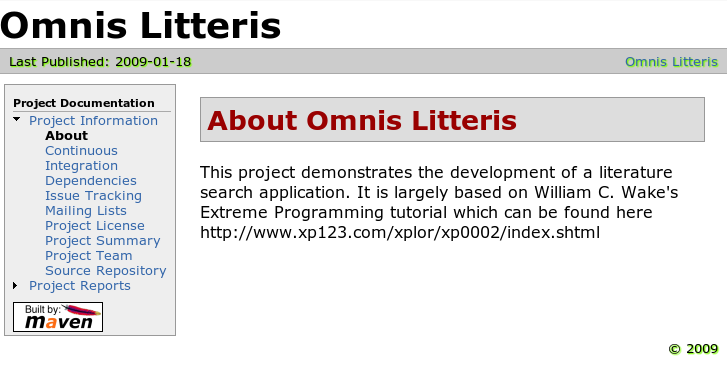
\includegraphics[width=\linewidth]{config-management/mvnsite}
\caption{Eine mit Maven erstellte Projektseite}
\end{figure}
\newslide
Für eine umfassende Dokumentation sorgen zahlreiche Plugins (Beispiele):
\begin{itemize}
\item Change-Log: maven-changelog-plugin
\item Checkstyle: maven-checkstyle-plugin
\item Junit-Report: maven-surefire-report-plugin
\item PMD: maven-pmd-plugin
\item Findbugs: findbugs-maven-plugin
\item JavaDoc: maven-javadoc-plugin
\item Cobertura: cobertura-maven-plugin
\item JXR (Cross-Reference): maven-jxr-plugin
\end{itemize}
\newslide
\begin{lstlisting}[language=xml,
  morekeywords={reporting,plugins,plugin,groupId,artifactId,
    version,configuration}]
  <reporting>
    <plugins>
      <plugin>
	<groupId>org.codehaus.mojo</groupId>
	<artifactId>cobertura-maven-plugin</artifactId>
      </plugin>
      <plugin>
	<artifactId>maven-javadoc-plugin</artifactId>
      </plugin>
      <plugin>
	<artifactId>maven-jxr-plugin</artifactId>
      </plugin>
 ..
    </plugins>
  </reporting>
\end{lstlisting}
\newslide
%\newpage
\newslide
\subsection{Eigene Dateien hinzufügen}
Das (lokale) Maven-Repository kann auch mit eigenen Dateien oder solchen,
die man von dritter Seite erhalten hat, ergänzt werden:
\begin{lstlisting}
mvn install:install-file     \
     -Dfile=Sample.jar       \
     -DgroupId=uniquesample  \
     -DartifactId=sample_jar \
     -Dversion=2.1.3b2       \
     -Dpackaging=jar         \
     -DgeneratePom=true
\end{lstlisting}
%
\newslide
\subsection{Software Version Control (SCM)}
Mit Hilfe des Plugins \verb+maven-scm-plugin+
bietet Maven auch eine einheitliche Schnittstelle zu
den Source-Code-Management (SCM) Systemen CVS, SVN, GIT (u.a.) an:
\begin{center}
\begin{tabular}{l|l}
Aktion & Beschreibung\\
\hline
 scm:checkin & Änderungen zum SCM-Repository senden\\
 scm:checkout & Arbeitskopie erstellen\\
 scm:add     & Datei hinzufügen\\
 scm:update  & Dateien aktualisieren \\
 scm:status & Status anzeigen\\
 scm:tag    & eine Markierung setzen\\
 \ldots
\end{tabular}
\end{center}
Bei einigen Aktionen müssen Parameter angegeben werden:
\begin{lstlisting}
  % mvn -Dmessage="<checkin comment here>" scm:checkin
\end{lstlisting}
Dazu muss in der POM-Datei das Element scm definiert werden:
\begin{lstlisting}[language=xml,
  morekeywords={scm,connection,developerConnection,url}]
<scm>
  <developerConnection>
    scm:svn:https://somerepository.com/svn_repo/trunk
  </developerConnection>
</scm>
\end{lstlisting}
Bei GIT lautet die URL wie folgt (Beispiel):
\begin{lstlisting}
  scm:git:git://github.com/path_to_repository
\end{lstlisting}
Weitere Infos: \href{http://maven.apache.org/scm/git.html}
                    {maven.apache.org/scm/git.html}
\newslide
\subsection{Release-Bildung}
Bei der Release-Bildung überprüft das Release-Plugin die folgenden Punkte:
\begin{itemize}
\item Sind alle lokalen Änderungen mit dem SCM-Repository abgeglichen?
\item Sind alle Integrations-Tests fehlerfrei durchgelaufen?
\item Werden bei den verwendeten Bibliotheken und Plugins
  keine SNAPSHOT-Versionen referenziert?
\end{itemize}
und sorgt dafür, dass die Versionsbezeichner in den POM-Dateien
entsprechend angepasst werden und mit den SCM-Tags korrespondieren:
\begin{lstlisting}
mvn release:prepare -DdryRun=true
\end{lstlisting}
\newslide
Das Plugin verlangt anschliessend die folgenden Angaben:
\begin{itemize}
\item aktueller Versionsbezeichner (Bsp: 1.0)
\item aktueller Releasebezeichner (Bsp: myapp-1.0)
\item neuer Bezeichner der Entwicklungsversion (Bsp: 1.1-SNAPSHOT)
\end{itemize}
und legt die eingebenen Werte in der Datei release.properties
ab. Zusätzlich werden verschiedene POM-Dateien erzeugt, die man
allesamt mit
\begin{lstlisting}
mvn release:clean
\end{lstlisting}
wieder löschen muss, wenn Maven die Aktionen ausführen soll.
\newslide
Nach Eingabe von
\begin{lstlisting}
mvn release:prepare
\end{lstlisting}
% achtung: bei SVN 1.5.2:
%    svn: Commit failed (details follow):
%    svn: File '..' already exists
%
% svn update und ein erneutes mvn:prepare behebt das Problem
%
wird Maven den aktuellen Stand des Projektes in das Tags-Verzeichnis
kopieren, die neue Versionsbezeichnung
in den POM-Dateien einsetzen und mitteilen, dass man nun mit
\begin{lstlisting}
mvn release:perform
\end{lstlisting}
die eigentlichen Release-Dateien bilden und in das lokale (und
Deploy-) Repository
transferieren kann. Damit dieser Schritt klappt, muss das
distributionManagement-Element definiert sein.
% Achtung:
% maven-release-plugin
% configuration tag
%  <plugin>
%        <artifactId>maven-release-plugin</artifactId>
%        <configuration>
%          <tagBase>http://localhost/omnislitteris/tags
%          </tagBase>
%        </configuration>
%      </plugin>
%

Eine verbesserte Unterstützung bietet das Plugin jgitflow:
\begin{lstlisting}[language=xml,morekeywords={plugin,groupId,artifactId,configuration,noDeploy}]
<plugin>
   <groupId>external.atlassian.jgitflow</groupId>
   <artifactId>jgitflow-maven-plugin</artifactId>
   <version>1.0-m5.1</version>
   <configuration>
     <noDeploy>true</noDeploy>
   <configuration>
</plugin>
\end{lstlisting}
Plugin goals:
\begin{itemize}
\item \structure{jgitflow:release-start} create and push a release branch
\item \structure{jgitflow:release-finish} build, tag and merge the release branch
into master and develop branches
\end{itemize}
\newslide
\subsection{Exercise}
\begin{enumerate}
\item Konvertieren Sie das Projekt Histogram in ein Maven-Projekt
(artifactId: histogram, groupId=demo) und
erstellen Sie die ausführbare Archiv-Datei mit allen benötigten Klassen.
Wie lautet der Dateiname der Archiv-Datei, und wie kann man ihn
konfigurieren?

%Hinweis: Bis und mit Version 1.0.12
%wird von jfreechart  die Library gnujaxp benötigt, welche
%nicht im offiziellen Maven-Repository abgelegt ist. Sie müssen
%in diesem Fall Ihre
%POM-Datei mit dem folgenden Repositories-Element ergänzen:
%\begin{lstlisting}[language=xml,
%   morekeywords={repositories,repository,id,name,url}]
%  <repositories>
%    <repository>
%      <id>maven-repository.atlassian.com</id>
%      <name>Atlassian Maven Repository</name>
%      <url>http://maven.atlassian.com/repository/public</url>
%    </repository>
%  </repositories>
%\end{lstlisting}
\end{enumerate}
%
\subsection{Software and further Informations}
\begin{itemize}
\item Maven: \href{http://maven.apache.org/}{maven.apache.org/}
\item Maven, The Definitive Guide
%(Tim O'Brien, John Casey, Brian Fox, Bruce Snyder, Jason Van Zyl)

\href{http://www.sonatype.com/book/reference/public-book.html}
{www.sonatype.com/book/reference/public-book.html}

\item Eclipse und Maven:
  \href{http://www.eclipse.org/m2e/}{www.eclipse.org/m2e/}
%\item An introduction to Maven 2
%
%\href{http://www.javaworld.com/javaworld/jw-12-2005/jw-1205-maven.html}
%   {www.javaworld.com/javaworld/jw-12-2005/jw-1205-maven.html}
%
%\item Building Web Applications with Maven
%
%   \href{http://today.java.net/pub/a/today/2007/03/01/building-web-applications-with-maven-2.html}
%      {today.java.net/pub/a/today/2007/03/01/building-web-applications-with-maven-2.html}
%
%\item Maven 2.0: Compile, Test, Run, Deploy, and More
%
%\href{http://www.onjava.com/pub/a/onjava/2006/03/29/maven-2-0.html}
%{www.onjava.com/pub/a/onjava/2006/03/29/maven-2-0.html}
%
%\item Get the most out of Maven 2 site generation:
%
%\href{http://www.javaworld.com/javaworld/jw-02-2006/jw-0227-maven.html}
%  {www.javaworld.com/javaworld/jw-02-2006/jw-0227-maven.html}
%
%\item Introduction to Apache Maven 2
%
%\href{http://www-128.ibm.com/developerworks/edu/j-dw-java-mavenv2.html}
%   {www-128.ibm.com/developerworks/edu/j-dw-java-mavenv2.html}
%
%\item Tutorial:Hibernate, Spring, HSQL, Eclipse \& Maven
%
%\href{http://www.lulu.com/content/1087191}{www.lulu.com/content/1087191}
%
%\item Netbeans Wiki: Maven best practices
%
%\href{http://wiki.netbeans.org/MavenBestPractices}
%  {wiki.netbeans.org/MavenBestPractices}
%
%\item Working with Maven in Netbeans
%
%\href{http://today.java.net/article/2009/10/14/working-maven-netbeans-671}
%  {today.java.net/article/2009/10/14/working-maven-netbeans-671}
\end{itemize}

\newpage

\section{Gradle}

Gradle is a build automation tool for multi-language software development.
It controls the development process in the tasks of compilation and
packaging to testing, deployment, and publishing.
Supported languages include Java (Kotlin, Groovy, Scala),
C/C++, and JavaScript.\\

Gradle builds on the concepts of Apache Ant and
Apache Maven, and introduces a Groovy- \verb|&| Kotlin-based domain-specific
language contrasted with the XML-based project configuration used by
Maven. Gradle uses a directed acyclic graph to determine the order
in which tasks can be run, through providing dependency management.\\

Gradle was designed for multi-project builds, which can grow to be large.
It operates based on a series of build tasks that can run serially or in
parallel. Incremental builds are supported by determining the parts of
the build tree that are already up to date; any task dependent only on
those parts does not need to be re-executed. It also supports caching
of build components, potentially across a shared network using the
Gradle Build Cache. It produces web-based build visualization called
Gradle Build Scans. The software is extensible for new features and
programming languages with a plugin subsystem.\\

Gradle is distributed as open-source software under the Apache License 2.0,
and was first released in 2007.
